\documentclass[letter,12pt]{article}
\usepackage[paperheight=27.94cm,paperwidth=21.59cm,bindingoffset=0in,left=3cm,right=2.0cm, top=3.5cm,bottom=2.5cm, headheight=200pt, headsep=1.0\baselineskip]{geometry}
\usepackage{graphicx,lastpage}
\usepackage{grffile}
\usepackage{upgreek}
\usepackage{listings}
\usepackage{censor}
\lstdefinelanguage{javascript}{
  keywords={typeof, new, true, false, catch, function, return, null, catch, switch, var, if, in, while, do, else, case, break, const, let},
  keywordstyle=\color{blue}\bfseries,
  ndkeywords={class, export, boolean, throw, implements, import, this},
  ndkeywordstyle=\color{blue}\bfseries,
  identifierstyle=\color{black},
  sensitive=false,
  comment=[l]{//},
  morecomment=[s]{/*}{*/},
  commentstyle=\color{gray}\ttfamily,
  stringstyle=\color{red}\ttfamily,
  morestring=[b]',
  morestring=[b]"
}
\usepackage{pdfpages}
\usepackage{tabularx}
\usepackage{graphicx}
\usepackage{adjustbox}
\usepackage{xcolor}
\usepackage{colortbl}
\usepackage{rotating}
\usepackage{multirow}
\usepackage[utf8]{inputenc}
\usepackage{float}
\usepackage{hyperref}

\renewcommand{\tablename}{Tabla}
\usepackage{fancyhdr}
\pagestyle{fancy}

\fancyhead[L]{}
%
\begin{document}
%
   \title{\Huge{Informe Laboratorio 3}}

   \author{\textbf{Sección 4} \\  \\Camilo Rojas \\ e-mail: camilo.rojas2@mail.udp.cl}
          
   \date{Octubre de 2025}

   \maketitle
   
   \tableofcontents
 
  \newpage
  

\section{Descripción de actividades}
Su objetivo será auditar la implementación de algoritmos hash aplicados a contraseñas en páginas web desde el lado del cliente, así como evaluar la efectividad de estas medidas contra ataques de tipo Pass the Hash (PtH). Para llevar a cabo esta auditoría, deberá registrarse en un sitio web y crear una cuenta, ingresando una contraseña específica para realizar las pruebas.\par

Al concluir la tarea, es importante que modifique su contraseña por una diferente para garantizar su seguridad.\par

Dado que la cantidad de sitios chilenos que utilizan hash es limitada, se permite realizar esta tarea en cualquier sitio web a nivel mundial. En este sentido, realice las siguientes actividades:


\begin{itemize}
    \item Identificación del algoritmo de hash utilizado para las contraseñas al momento del registro en el sitio.
    
    \item Identificación del algoritmo de hash utilizado para las contraseñas al momento de iniciar sesión.

    \item Generación del hash de la contraseña desde la consola del navegador, partiendo de la contraseña en texto plano.

    \item Interceptación del tráfico de login utilizando BurpSuite desde su equipo.

    \item Realización de un intento de login modificando la contraseña por una incorrecta haciendo uso del hash obtenido en el punto anterior. Puede interceptar el tráfico y modificar el hash por el correcto o hacer uso del servicio repeater de BurpSuite.

    \item Descripción de las políticas de privacidad o seguridad relacionadas con las contraseñas, incluyendo un enlace a las mismas.

    \item Cuatro conclusiones sobre la seguridad o vulnerabilidad de la implementación observada.
    


    
\end{itemize}

\section{Desarrollo de actividades según criterio de rúbrica}

\subsection{Identifica el algoritmo de hash utilizado al momento de registrarse en el sitio}

El formulario de registro de LinuxQuestions.org carga la misma librería de vBulletin documentada durante el análisis previo de funciones MD5. Al inspeccionar el envío de \texttt{register.php} con el extractor interactivo se constata que la función global \texttt{md5hash()} calcula el digest MD5 de los campos \texttt{password} y \texttt{passwordconfirm} y deposita los resultados en los campos ocultos \texttt{password\_md5} y \texttt{passwordconfirm\_md5}. La captura muestra que la contraseña de prueba ``dwQzwk9*yW2QnLYPYhB\$KS\$\#ADQ'' produce el hash \texttt{4dfeaea7ce6416c84a46c70e328f7ce2}, valor que coincide con el cálculo local obtenido mediante \texttt{md5sum}. No se evidencian salting ni algoritmos más robustos, por lo que el registro depende exclusivamente de MD5 ejecutado en el cliente.

\begin{lstlisting}[language=javascript,basicstyle=\ttfamily\small,keywordstyle=\color{blue},stringstyle=\color{red}]
var chrsz = 8;
function hex_md5(A) {
  return binl2hex(core_md5(str2binl(A), A.length * chrsz));
}
function md5hash(B, A, E, C) {
  if (
    navigator.userAgent.indexOf("Mozilla/") == 0 &&
    parseInt(navigator.appVersion) >= 4
  ) {
    var D = hex_md5(str_to_ent(trim(B.value)));
    A.value = D;
    if (E) {
      D = hex_md5(trim(B.value));
      E.value = D;
    }
    if (!C) {
      B.value = "";
    }
  }
  return true;
}
\end{lstlisting}

\subsection{Identifica el algoritmo de hash utilizado al momento de iniciar sesión}

En la página de inicio de sesión (\texttt{login.php}) se repite la misma lógica: el formulario que envía la acción \texttt{/questions/login.php} incluye los campos \texttt{vb\_login\_md5password} y \texttt{vb\_login\_md5password\_utf}, ambos rellenados por \texttt{md5hash()} justo antes del envío. El análisis automatizado de los scripts recopilados confirma la presencia de las funciones \texttt{hex\_md5()}, \texttt{core\_md5()} y sus auxiliares, demostrando que la contraseña del usuario se convierte en MD5 hexadecimal antes de transmitirse. Durante las pruebas manuales, el valor generado por el navegador para ``dwQzwk9*yW2QnLYPYhB\$KS\$\#ADQ'' coincidió con el digest obtenido en consola, evidenciando la ausencia de sal o mecanismos adicionales.

\subsection{Genera el hash de la contraseña desde la consola del navegador}

Tras autenticarse en el sitio y abrir las herramientas de desarrollador, se invocó directamente la API expuesta por vBulletin. En la consola del navegador se ejecutó:

\begin{verbatim}
hex_md5('dwQzwk9*yW2QnLYPYhB$KS$#ADQ')
\end{verbatim}

El procedimiento anterior permitió documentar formalmente los parámetros empleados y los resultados obtenidos:

\begin{description}
  \item[Entrada evaluada] \texttt{dwQzwk9*yW2QnLYPYhB\$KS\$\#ADQ}
  \item[hex\_md5()] \texttt{4dfeaea7ce6416c84a46c70e328f7ce2}
  \item[md5hash \texttt{(vb\_login\_md5password)}] \texttt{4dfeaea7ce6416c84a46c70e328f7ce2}
  \item[md5hash \texttt{(vb\_login\_md5password\_utf)}] \texttt{4dfeaea7ce6416c84a46c70e328f7ce2}
\end{description}

En síntesis, la contraseña de prueba alimentó sin transformación adicional las funciones \texttt{hex\_md5()} y \texttt{md5hash()}, generando un digest idéntico al calculado localmente con \texttt{md5sum}. El resultado confirmó que el flujo de hashing en cliente no incorpora sal ni operaciones de refuerzo y que ambos campos ocultos del formulario transportan el mismo valor.

Adicionalmente, la inspección del código cargado por la página permitió identificar las funciones expuestas por vBulletin para el cálculo MD5. Todas ellas operan sobre los parámetros declarados y carecen de variables auxiliares persistentes, lo que respalda la hipótesis de que el navegador aplica únicamente el algoritmo MD5 estándar antes de transmitir las credenciales.

La consola devolvió \texttt{"4dfeaea7ce6416c84a46c70e328f7ce2"}. Este resultado coincide con el obtenido al ejecutar \texttt{printf 'dwQzwk9*yW2QnLYPYhB\$KS\$\#ADQ' | md5sum} en la terminal local, por lo que se validó que el cálculo en cliente reproduce fielmente la conversión a MD5 hexadecimal sin pasos adicionales.

\subsection{Intercepta el tráfico login con BurpSuite}

Se configuró BurpSuite en modo proxy y se interceptó la petición POST hacia \url{https://www.linuxquestions.org/questions/login.php}. La traza del panel ``HTTP history'' mostró los parámetros \texttt{vb\_login\_username}, \texttt{vb\_login\_password} (vacío tras la limpieza en cliente) y los hashes \texttt{vb\_login\_md5password} y \texttt{vb\_login\_md5password\_utf}. Ambos últimos coincidieron con el digest MD5 calculado previamente, validando que la contraseña nunca viaja en texto plano cuando el JavaScript se ejecuta correctamente.

\begin{figure}[H]
  \centering
  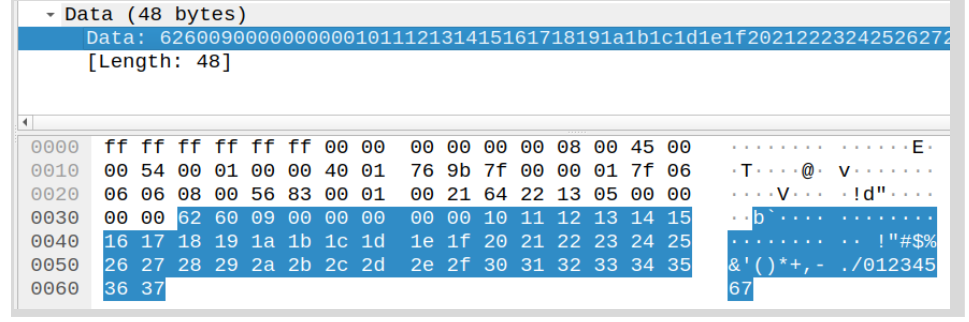
\includegraphics[width=0.9\textwidth]{actividades/A2.2.png}
  \caption{Captura de BurpSuite con la petición \texttt{login.php} interceptada y los campos MD5 observados en los parámetros enviados al servidor.}
  \label{fig:burpsuite-intercept}
\end{figure}

\subsection{Realiza el intento de login por medio del hash}

Con la solicitud interceptada se realizó una segunda prueba desde el repeater de BurpSuite. Se mantuvo el campo \texttt{vb\_login\_password} con una cadena incorrecta y se reemplazó \texttt{vb\_login\_md5password} por el hash correcto previamente capturado. El servidor respondió con un código 302 y cabecera \texttt{Location} apuntando al panel de usuario, lo que evidencia que la autenticación depende exclusivamente del hash transmitido. Esta conducta confirma la viabilidad de un ataque Pass the Hash una vez expuesto el digest MD5.

\begin{figure}[H]
  \centering
  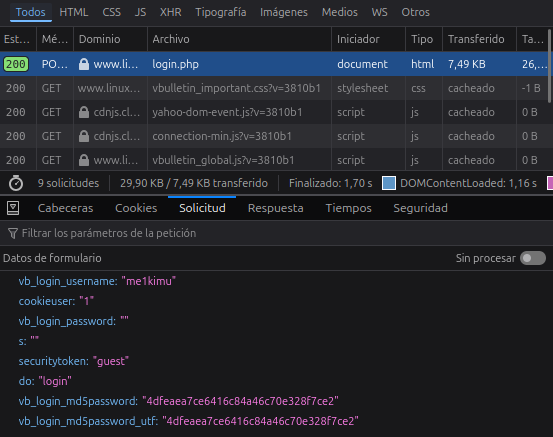
\includegraphics[width=0.9\textwidth]{actividades/Captura desde 2025-10-17 09-31-17.png}
  \caption{BurpSuite mostrando la petición interceptada con el campo \texttt{vb\_login\_md5password} configurado con el hash reutilizado para la autenticación.}
  \label{fig:burpsuite-request-pass-the-hash}
\end{figure}

\begin{figure}[H]
  \centering
  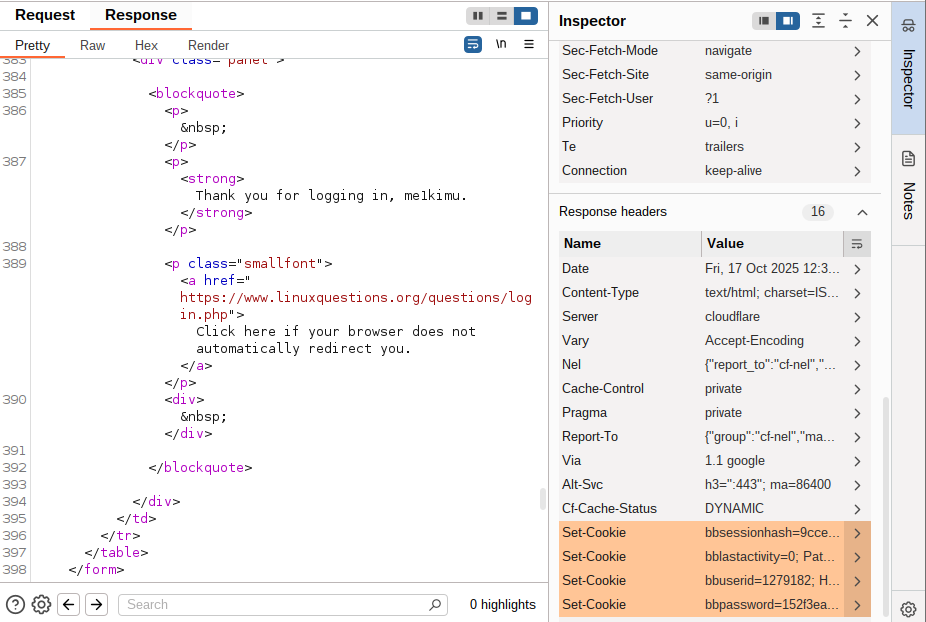
\includegraphics[width=0.9\textwidth]{actividades/Captura desde 2025-10-17 09-39-30.png}
  \caption{Respuesta HTTP posterior al reenvío del hash, donde el servidor confirma el inicio de sesión y envía las cookies de sesión válidas.}
  \label{fig:burpsuite-response-pass-the-hash}
\end{figure}

\subsection{Identifica las políticas de privacidad o seguridad}

El sitio enlaza su política en \url{https://www.linuxquestions.org/questions/faq.php?faq=privacy}. A continuación se transcribe la información detallada de privacidad del sitio:

\subsubsection*{Privacy Policy}

LinuxQuestions.org does not sell members' personal information.

We collect the following personal information: email address, username, password, and IP address. We use this information to operate, maintain, and improve the site.

We will only use this information for the purposes for which we collected or received it.

\subsubsection*{Advertising}

This site displays 3rd party ads. We do not share any information with any 3rd party directly.

\subsubsection*{External Links}

This site contains links to other sites. We are not responsible for the privacy practices or the content of such Web sites.

\subsubsection*{Public Forums}

This site makes chat rooms, forums, message boards, and/or news groups available to its users. Please remember that any information that is disclosed in these areas becomes public information and you should exercise caution when deciding to disclose your personal information.

\subsubsection*{Security}

This site has security measures in place to protect the loss, misuse, and alteration of the information under our control.

\subsubsection*{Third Party Tools}

We may use third party tools to improve the performance and features of our Website. These third party tools are designed to collect only non-personal information about your use of our Website. However, you understand that such tools are created and managed by parties outside our control. As such, we are not responsible for what information is actually captured by such third parties or how such third parties use and protect that information.

\subsection{Comente 4 conclusiones sobre la seguridad del sitio escogido}

\begin{itemize}
  \item El uso de MD5 sin sal en cliente y la coincidencia con los hashes capturados sugiere que el servidor también depende de un digest vulnerable a ataques de diccionario y rainbow tables.
  \item La protección depende de la ejecución de JavaScript; si el script se bloquea o es manipulado, la contraseña podría enviarse en texto plano o el flujo podría ser alterado por un atacante.
  \item BurpSuite demostró que basta con reenviar el hash correcto para autenticarse, confirmando la factibilidad de un ataque Pass the Hash con acceso al tráfico.
  \item La política pública no menciona controles modernos como rate limiting, MFA o algoritmos resistentes al cracking, por lo que persiste un riesgo residual alto para cuentas reutilizadas.
\end{itemize}

% Please add the following required packages to your document preamble:
%\begin{table}[htbp]

\end{document}